% \documentclass[landscape,a0b,final]{a0poster}
\documentclass[landscape,a0b,final,a4resizeable]{a0poster}

%%% Option "a4resizeable" makes it possible ot resize the
% poster by the command: psresize -pa4 poster.ps poster-a4.ps
% For final printing, please remove option "a4resizeable" !!
% \usepackage[a0paper]{geometry}
\usepackage[dvips]{graphicx}
\usepackage{epsfig}
\usepackage{color}
\usepackage{shadow}
\usepackage{multicol}
\usepackage{times}
% \usepackage{pstricks}
\usepackage{algorithmic}
% \usepackage{algorithm}
% \usepackage{subfigure}}
% \usepackage{amsmath}
% \usepackage{amssymb}
% \usepackage{url}
\usepackage{sectsty}
\usepackage{definitions}
% \usepackage[absolute]{textpos}
\usepackage[it]{subfigure}
\usepackage{booktabs}
\usepackage{multirow}
\usepackage{setspace}
\usepackage[scaled=0.8]{DejaVuSansMono}

%%% Size of Poster etc.
\newlength{\textArea}
\setlength{\textArea}{90cm}  % for a0b = A0-big !!
\setlength{\columnsep}{3cm}
\setlength{\columnseprule}{2mm}
\setlength{\parindent}{0.0cm}



%%%%%%%%%%%%%%%%%%%%%%%%%%%%%%%%%%%%%%%%%%%%%%%%%%%%%%%%%%%%%%%%%%%%%%%%%%%%%%%% 
%%% Begin of Document
\renewcommand{\normalsize}{\large}
\begin{document}
\definecolor{backgroundCol}{rgb}{1,1,1} % Cardiff yellow
\pagecolor{backgroundCol}

%%%%%%%%%%%%%%%%%%%%%%%%%%%%%%%%%%%%%%%% 
% Definition of Colors
% Background- and Text-color
% \definecolor{mainCol}{rgb}{0.91,0.91,1}
% \definecolor{TextCol}{rgb}{0,0,0}
% \definecolor{mainCol}{rgb}{0.839,0.212,0.2784}% 214 54 71
% \definecolor{mainCol}{rgb}{0.8549,0.2196,0.2824}% 214 54 71
\definecolor{mainCol}{rgb}{0.8078,0.0196,0.2235}% According to the website
\definecolor{TextCol}{rgb}{1,1,1}
\definecolor{black}{rgb}{0,0,0}

\setlength{\sboxrule}{2pt}
\setlength{\sboxsep}{0pt}

\vspace*{0cm}
%%% Title und Author
%%% University-emblem
% \shabox{%
  % \hfill
% \shabox{%
    \begin{minipage}[c][0.12\textArea][c]{0.3\textArea}
      % \begin{center}
      \vspace{1cm}
      
\includegraphics[width=0.3\textArea]{comsc}
      \nobreak
      % \end{center}
    \end{minipage}
  \colorbox{white}{
    \begin{minipage}[c][0.12\textArea][c]{0.7\textArea}
      \begin{center}
        \textcolor{mainCol}{
          {\VeryHuge NONHOLONOMIC ROUTE PLANNING\\\vspace{0.5ex}FOR DRIVERLESS RACING}
          % \vspace{1cm}
          % {\Large Matteo de Rosa$^{1}$, Kirill Sidorov$^{1}$,
          %   He Wang$^{2}$,
          %   Peter Sandilands$^{2}$,
          %   Taku Komura$^{2}$}\\
          % \qquad
          % \Large{School of Computer Science and Informatics,
          %   School of Enigneering, Cardiff University}\\
          %   \large{E-mail: \texttt{SidorovK@cardiff.ac.uk}}}\\
          }%
      \end{center}
    \end{minipage}
  }
  % \colorbox{white}{
  % }
\hfill
% \shabox{
\colorbox{white}{
    \begin{minipage}[c][0.12\textArea][c]{0.24\textArea}
      % \begin{center}
      \vspace{1cm}
      
\includegraphics[width=0.24\textArea]{cr}
      \nobreak
      % \end{center}
    \end{minipage}
  }
% }
    % \hfill
%%% University-emblem
% }%\vspace{2cm}
% vspace{2cm}


%%% Begin of Multicols-Enviroment
\begin{multicols}{4}


  %%% Introduction
  \mysection{Introduction}
\begin{minipage}{\linewidth}
\begin{figurehere}
  \centering
  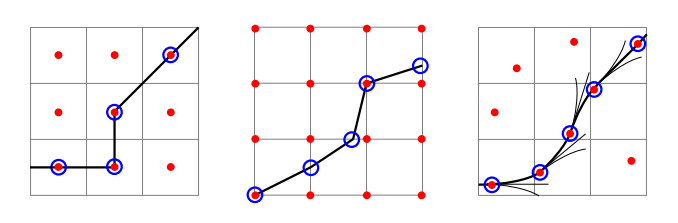
\includegraphics[width=1\linewidth]{img/comparison}
  \vspace{-2em}
  \mycaption{Comparison of search algorithms. Nodes are represented by the red
    dots. \emph{Left:} A*, \emph{centre:} D*, \emph{right:} hybrid-state A*. [4]}
  \label{fig:comparison}
\end{figurehere}
\vspace{-0.5em}
\end{minipage}

\mysection{Hybrid-State A\**}
Path is composed of arcs subject to the following constraints:
\begin{itemize}
\item The distance travelled $d$ has to be enough to exit the cell. For a cell of
  $d \ge \sqrt{2}\cdot s$ for a cell of size $s$.
  \item The curvature is restricted by the maximum vehicle steering angle $\alpha$.
\end{itemize}

\mysection{Results and Evaluation}
\begin{minipage}{\linewidth}
\begin{figurehere}
  \centering
  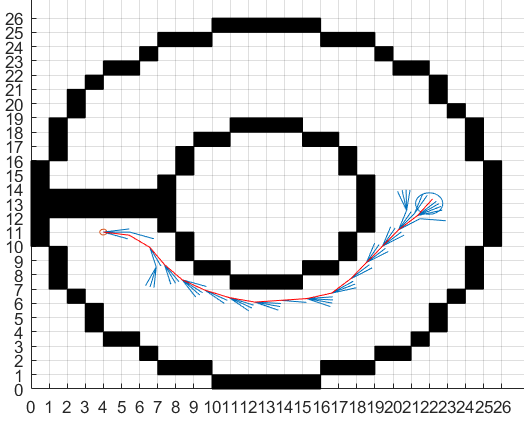
\includegraphics[width=0.49\linewidth]{img/half}
  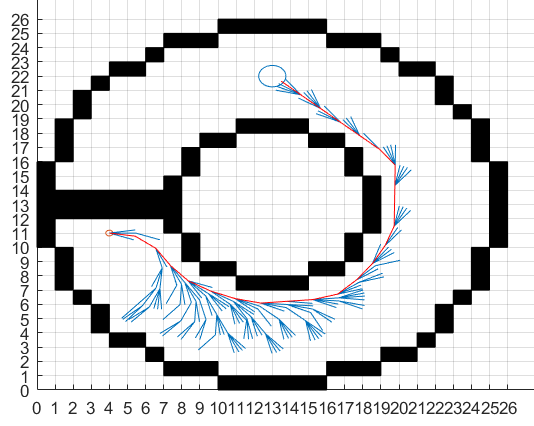
\includegraphics[width=0.49\linewidth]{img/three_quarters}
  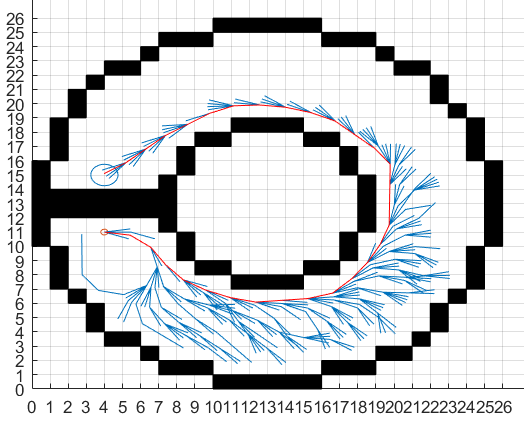
\includegraphics[width=0.49\linewidth]{img/full}
  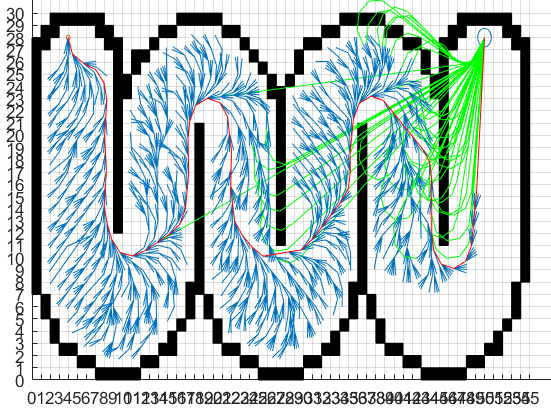
\includegraphics[width=0.49\linewidth]{img/snake}
  \raisebox{10ex}{\begin{minipage}{0.49\linewidth}
    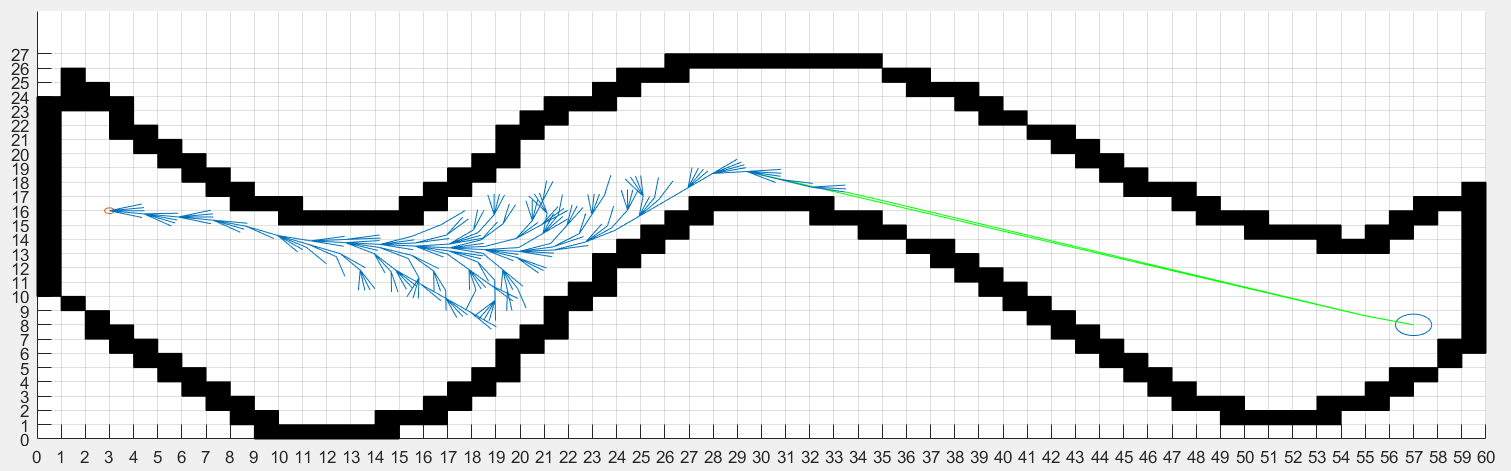
\includegraphics[width=1\linewidth]{img/long_snake}
    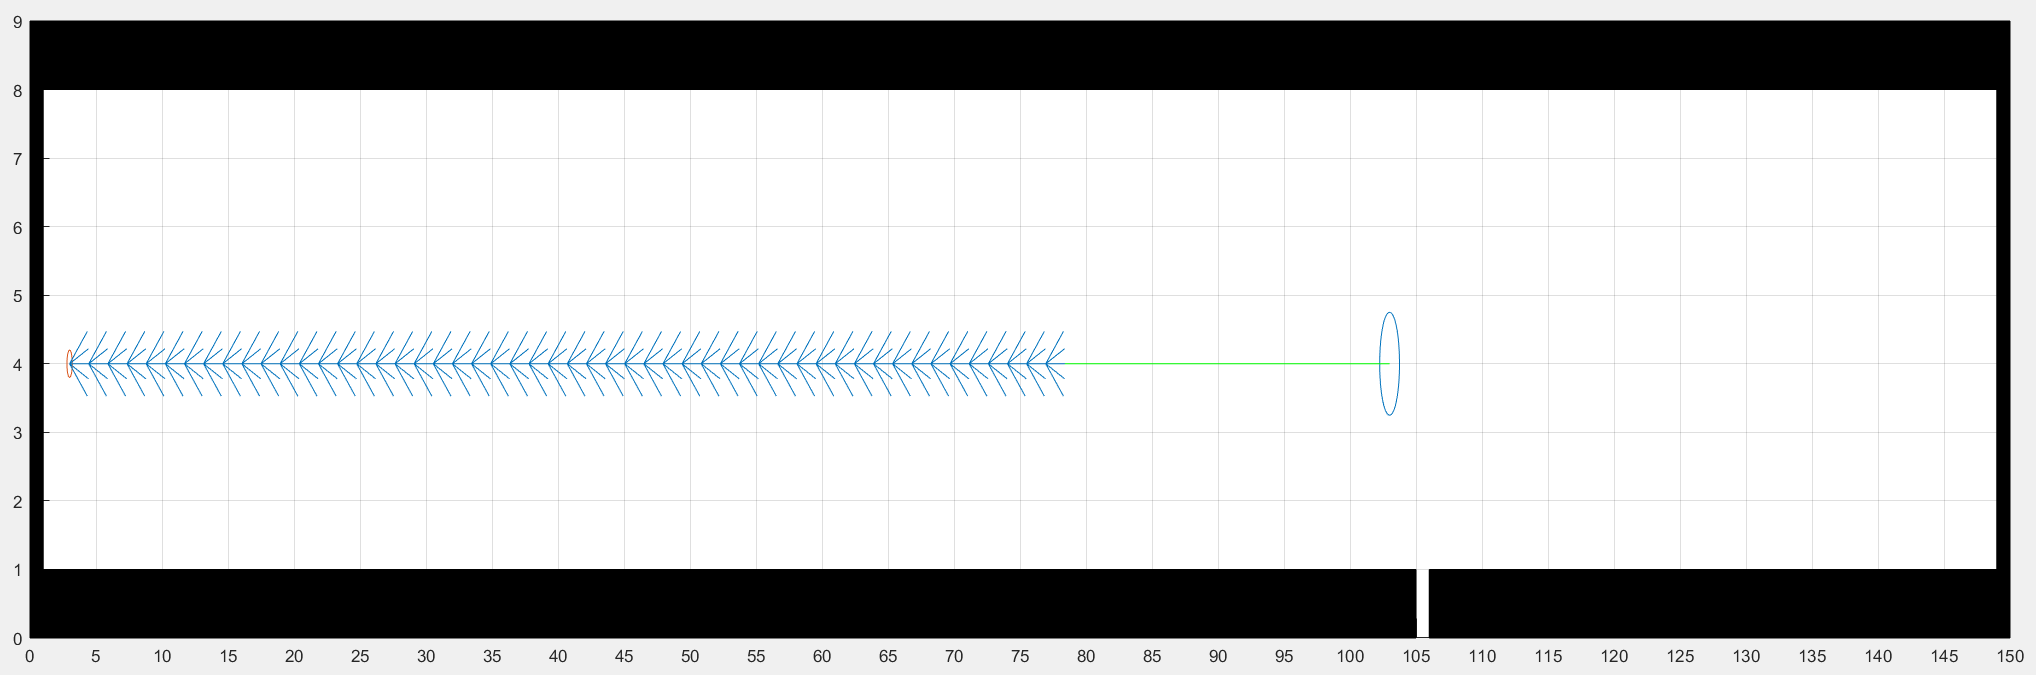
\includegraphics[width=1\linewidth]{img/trivial}
  \end{minipage}}
  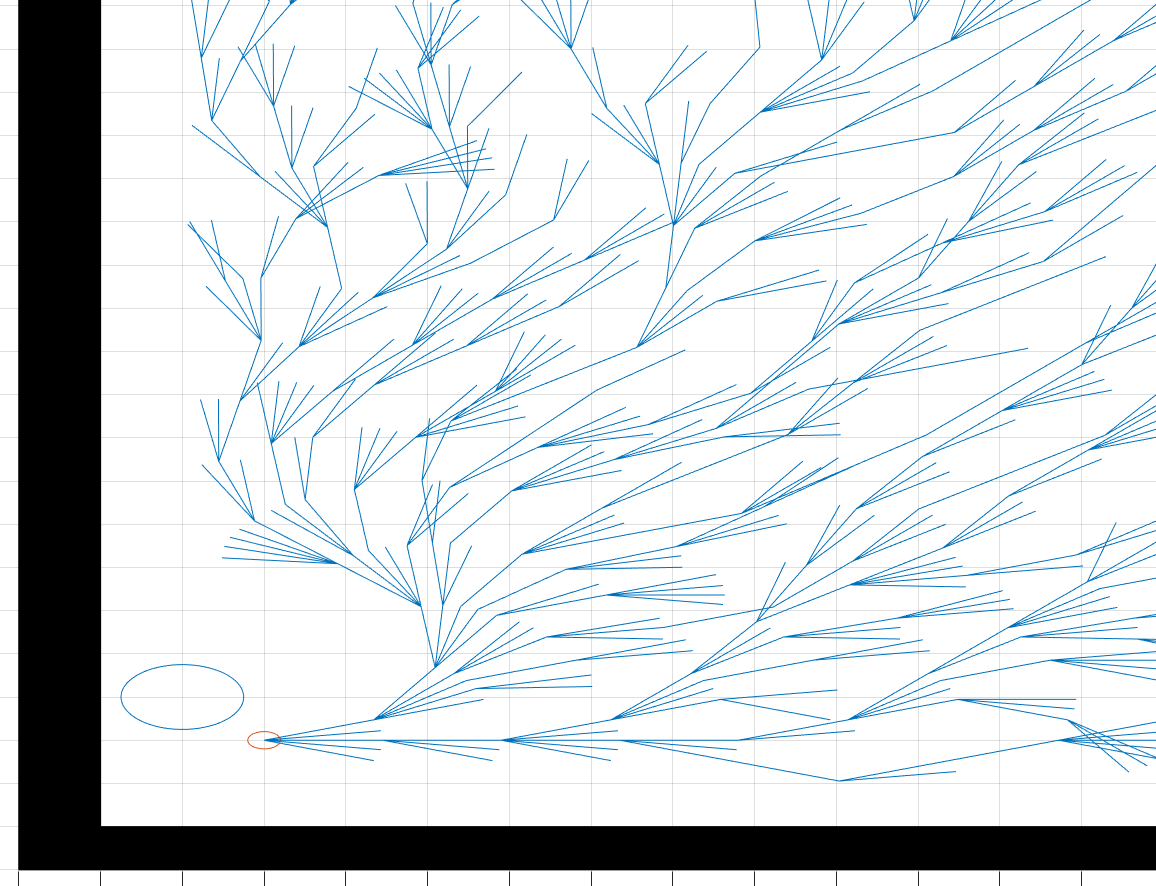
\includegraphics[width=0.49\linewidth]{img/empty}
  \vspace{-2em}
  \label{fig:comparison}
\end{figurehere}
\vspace{-0.5em}
\end{minipage}


  % -------------------------------------------------------------------------

  \mysection{References}
  {
    \small
    \bibliographystyle{ieee}
    \bibliography{thesis}
  }
\end{multicols}
\end{document}
